\documentclass[12pt]{article}
\usepackage[left=2cm,right=2cm,top=2cm,bottom=2cm,letterpaper]{geometry}
\usepackage{lmodern}
\usepackage[T1]{fontenc}
\usepackage[utf8]{inputenc}
\usepackage[spanish,activeacute]{babel}
\usepackage{hyperref}
\usepackage{graphicx}
\graphicspath{{graphic/}}
\usepackage{float}
\usepackage{caption}
\usepackage[toc]{multitoc}
\setcounter{tocdepth}{2}
% automata
\usepackage{tikz}
\usepackage{pmboxdraw} 

\title{Proyecto 2}
\author{Carlos Gerardo Acosta Hernández \\ Andrea Itzel González Vargas \\ Luis Pablo Mayo Vega}
\date{Redes de Computadoras\\Facultad de Ciencias, UNAM}
%\setlength{\parindent}{0em}
\begin{document}
\maketitle
\tableofcontents
\newpage
\section{Especificación de requerimientos}
\subsection{Enunciado del problema}
De acuerdo con el modelo TCP/IP, \textit{la Capa de Aplicación} es la de mayor importancia y en la que se sustenta todo el desarrollo de redes de computadoras pues está compuesta por los protocolos y demás servicios encargados de manejar, intercambiar o decodificar los datos que los usuarios se envían a través de distintos hosts para comunicarse. En otras palabras, se busca que dos o más procesos en distintas computadoras puedan ser capaces de intercambiar información y de esta manera otorgar una mayor capacidad de procesamiento y mejor rendimiento del que se tendría con un único host.\\

Sin embargo, la \textit{Capa de Aplicación} no puede trabajar sola, siendo mediante un proceso de encapsulación en cada una de las capas, que los datos(PDU) se envian a las capas inferiores, añadiendo cada una de las capas información que le concierne para que sus protocolos puedan manejarlos.\\

Como sabemos, protocolos como \textsf{HTTP, DNS, FTP, SMTP o DHCP} tienen cada uno una estructura distinta ya bien definida y estandarizada en los articulos de \textit{Request for Comments} publicados, pero eso no significa que sean los únicos protocolos disponibles en la \textit{Capa de Aplicación}. La gran ventaja de esta capa es su adaptabilidad para que se desarrollen protocolos de acuerdo a las necesidades de la aplicación sobre la que se usarán. 

\subsection{Objetivo de la aplicación}

Esta aplicación fue creada con el objetivo de implementar un protocolo de la capa de aplicación en el que el usuario, conectado del lado del cliente, solicite un pokémon a capturar. El servidor elegirá aleatoriamente alguno de los pokémon que estén en su base de datos, se lo ofrecerá al usuario y, si éste acepta capturarlo, también aleatoriamente se indicará
 si logró capturarlo o no. \\

 El usuario también podrá ser capaz de consultar su Pokédex, con los nombres de los pokémon que ha capturado y la imagen de cada pokémon que seleccione. \\

 El protocolo que hemos diseñado se enfocará en las acciones del usuario y el servidor que involucren una comunicación entre ambos, cada una con un tipo de mensaje específico. Es decir, si un usuario quisiera capturar un pokémon, solo tendría que  enviar un mensaje con el código que el servidor entienda como "quiero capturar un pokémon" sin considerar otros aspectos como el nombre del pokémon o el tamaño de la imagen que contiene a tal pokémon. \\

 En ese sentido, diseñar nuestro propio protocolo nos permite tener mayor control sobre la tasa de transferencia de los datos dentro de la aplicación, disminuyendo los costos de la comunicación y mejorando el desempeño del programa.

 \newpage
 \subsubsection{Casos de uso}
 \begin{center}
   \begin{tabular}{|l|p{5cm}|p{9cm}|}
     \hline
     Actor & Caso de uso & Descripción \\
     \hline
     Pokentrenador & Iniciar sesión & El usuario se conecta con el servidor y se le muestra el menú principal de la aplicación \\ \hline
     Pokentrenador & Capturar pokémon & El usuario solicita al servidor que le muestre un pokémon y decide si intenta capturarlo (con un número finito de intentos) o no\\ \hline
     Pokentrenador & Consultar pokedex & El usuario hace una consulta para buscar un pokémon en su pokédex \\ \hline
     Pokentrenador & Cerrar sesión & Cierra la conexión con el servidor \\
     \hline
   \end{tabular}
 \end{center}


 \begin{figure}[H]
   \centering
   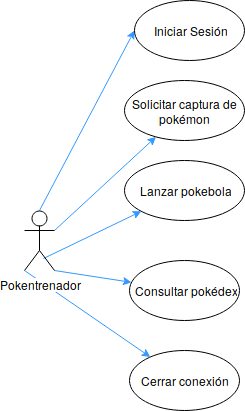
\includegraphics[width=0.4\textwidth]{casosdeuso}
   \caption{Diagrama de casos de uso de la aplicación}
 \end{figure}

 \newpage
\section{Diseño del protocolo}
\subsection{Máquina de Estados Finita}
Máquina de Estados Finita para el protocolo de la capa de aplicación.
\begin{center}
\begin{tikzpicture}[scale=0.2]
\tikzstyle{every node}+=[inner sep=0pt]
\draw [black] (7.7,-22) circle (3);
\draw (7.7,-22) node {$q_0$};
\draw [black] (21.9,-21.4) circle (3);
\draw (21.9,-21.4) node {$q_1$};
\draw [black] (35.4,-21.4) circle (3);
\draw (35.4,-21.4) node {$q_2$};
\draw [black] (63.3,-21.4) circle (3);
\draw (63.3,-21.4) node {$q_3$};
\draw [black] (35.4,-7.3) circle (3);
\draw (35.4,-7.3) node {$q_4$};
\draw [black] (63.3,-46.6) circle (3);
\draw (63.3,-46.6) node {$q_5$};
\draw [black] (35.4,-46.6) circle (3);
\draw (35.4,-46.6) node {$q_6$};
\draw [black] (7.7,-49.9) circle (3);
\draw (7.7,-49.9) node {$q_9$};
\draw [black] (9.968,-20.054) arc (121.77715:63.06187:9.706);
\fill [black] (19.48,-19.65) -- (18.99,-18.84) -- (18.54,-19.74);
\draw (14.59,-18.02) node [above] {$c:10$};
\draw [black] (24.9,-21.4) -- (32.4,-21.4);
\fill [black] (32.4,-21.4) -- (31.6,-20.9) -- (31.6,-21.9);
\draw (28.65,-21.9) node [below] {$s:20$};
\draw [black] (19.52,-23.209) arc (-61.01633:-114.14465:10.403);
\fill [black] (10.22,-23.6) -- (10.75,-24.39) -- (11.16,-23.47);
\draw (15,-25.09) node [below] {$s:44$};
\draw [black] (34.348,-24.204) arc (-26.53097:-150.98729:14.4);
\fill [black] (8.87,-24.76) -- (8.82,-25.7) -- (9.7,-25.21);
\draw (21.8,-32.71) node [below] {$c:11$};
\draw [black] (37.033,-9.805) arc (25.08093:-25.08093:10.722);
\fill [black] (37.03,-9.81) -- (36.92,-10.74) -- (37.82,-10.32);
\draw (38.54,-14.35) node [right] {$c:12$};
\draw [black] (34.029,-18.74) arc (-159.56755:-200.43245:12.574);
\fill [black] (34.03,-18.74) -- (34.22,-17.82) -- (33.28,-18.16);
\draw (32.74,-14.35) node [left] {$s:21/e:44$};
\draw [black] (38.4,-21.4) -- (60.3,-21.4);
\fill [black] (60.3,-21.4) -- (59.5,-20.9) -- (59.5,-21.9);
\draw (49.35,-21.9) node [below] {$c:13$};
\draw [black] (63.3,-24.4) -- (63.3,-43.6);
\fill [black] (63.3,-43.6) -- (63.8,-42.8) -- (62.8,-42.8);
\draw (62.8,-34) node [left] {$s:22$};
\draw [black] (38.199,-45.523) arc (108.58634:71.41366:34.985);
\fill [black] (38.2,-45.52) -- (39.12,-45.74) -- (38.8,-44.79);
\draw (49.35,-43.2) node [above] {$c:15$};
\draw [black] (60.488,-47.642) arc (-72.05358:-107.94642:36.146);
\fill [black] (60.49,-47.64) -- (59.57,-47.41) -- (59.88,-48.36);
\draw (49.35,-49.9) node [below] {$s:23$};
\draw [black] (35.4,-43.6) -- (35.4,-24.4);
\fill [black] (35.4,-24.4) -- (34.9,-25.2) -- (35.9,-25.2);
\draw (35.9,-34) node [right] {$s:24/e:41$};
\draw [black] (7.7,-25) -- (7.7,-46.9);
\fill [black] (7.7,-46.9) -- (8.2,-46.1) -- (7.2,-46.1);
\draw (7.2,-35.95) node [left] {$c:00$};
\draw [black] (61.07,-44.59) -- (37.63,-23.41);
\fill [black] (37.63,-23.41) -- (37.88,-24.32) -- (38.56,-23.58);
\draw (51.59,-33.51) node [above] {$c:14$};
\end{tikzpicture}
\end{center}

\subsection{Descripción de los estados}
\begin{center}
\begin{tabular}{|l|p{9cm}|}
  \hline
  Estado & Descripción \\
  \hline
  $q_0$ & Conexión establecida, inicio de aplicación. \\ \hline
  $q_1$ & Inicio de sesión. \\ \hline
  $q_2$ & Menú de juego. \\ \hline
  $q_3$ & Solicitud de captura de \textit{pókemon}. \\ \hline
  $q_4$ & Búsqueda de un pókemon en la \textit{pókedex}. \\ \hline
  $q_5$ & Aparición de un \textit{Pókemon} salvaje. \\ \hline
  $q_6$ & Intento de captura de \textit{pókemon}.\\ \hline
  $q_9$ & Cierre de conexión. \\
  \hline
\end{tabular}
\end{center}
\newpage

\subsection{Descripción de los mensajes en la comunicación cliente-servidor}
\begin{center}
  \begin{tabular}{|l|c|p{5.9cm}|}
    \hline
    Código & Segmento & Descripción \\ \hline
    \hline
    00 & \texttt{|long|code|} & Termina la conexión para un cliente. \\ \hline
    10 & \texttt{|long|code|name|} & Solicitud de inicio de sesión del cliente. El parámetro \texttt{name} se refiere al nombre de usuario del cliente. \\ \hline
    11 & \texttt{|long|code|} & Solicitud de cierre de sesión del cliente. \\ \hline
    12 & \texttt{|long|code|name|} & Acceso y consulta a la \textit{Pokédex} mediante el nombre de un pokémon. \\ \hline
    13 & \texttt{|long|code|} & Acceso a la opción de captura. \\ \hline
    14 & \texttt{|long|code|} & El usuario rechaza el pokémon salvaje ofrecido por el servidor. \\ \hline
    15 & \texttt{|long|code|attempts|name|} & Intento de captura del pokémon salvaje ofrecido. \\ \hline %%dfdishffjsjfsfvkfdjhJNDSJFNSDGLDKN
    \hline
    20 & \texttt{|long|code|} & Inicio de sesión del cliente exitoso. \\ \hline
    21 & \texttt{|long|code|long\_n|name|long\_img|img} & Resultado exitoso de la Pokédex con imagen del pokémon. \\ \hline %wat
    22 & \texttt{|long|code|attempts|name|} & Selección aleatoria de un pokémon salvaje para el cliente. Incluye el máximo número de intentos. \\ \hline
    23 & \texttt{|long|code|attempts|name|} & Pokémon no capturado, disminución del número de intentos. \\ \hline
    24 & \texttt{|long|code|long\_n|name|long\_img|img|} & Pokémon capturado con imagen incluída. \\ \hline \hline
    41 & \texttt{|long|code|} & Error: Máximo número de intentos de captura alcanzados. \\ \hline
    44 & \texttt{|long|code|} & Error: Consulta infructuosa. \\ \hline
  \end{tabular}
\end{center}

\subsection{Diseño de la base de datos}
 \begin{figure}[H]
   \centering
   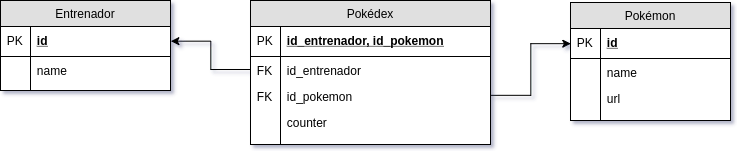
\includegraphics[width=1\textwidth]{PokeDB2}
   \caption{Diagrama de la base de datos relacional.}
 \end{figure}

\section{Implementación del protocolo}
\subsection{Especificación del ambiente de desarrollo}\label{sec:env}
%revisar versiones
\begin{tabular}{l r l r}
  \textbf{Lenguaje de programación:} & Java & \textbf{versión:} & 1.8 \\
  \textbf{Herramienta de construcción de software:} & Apache Ant & \textbf{versión:} & 1.9.9 \\
  \textbf{Sistema Manejador de Base de Datos:} & sqlite & \textbf{versión:} & 2.8.17 \\
  \textbf{Driver de conectividad JDBC:} & sqlite-jdbc & \textbf{versión:}& 3.16.1\\
  \textbf{Sistema manejador de versiones:} & GIT & \textbf{versión:}& 2.14.1 \\
  \textbf{Pruebas Unitarias:} & JUnit y Hamcrest & \textbf{versión:}& 4 \\
  
\end{tabular}

\subsection{Estructura del proyecto}
\subsubsection{Árbol del directorio (preinstalación)}
\begin{verbatim}
p02
├── build.xml
├── documentos
│   ├── graphic
│   │   ├── casosdeuso.png
│   │   └── ...
│   ├── proyecto2.pdf
│   └── proyecto2.tex
├── lib
│   ├── hamcrest-core.jar
│   ├── junit.jar
│   └── sqlite-jdbc-3.16.1.jar
├── man
│   └── proyecto2.1
├── src
│   ├── redes
│   │   ├── ClienteHilo.java
│   │   ├── ConexionBD.java
│   │   ├── Controlador.java
│   │   ├── Estado.java
│   │   ├── FabricaMensaje.java
│   │   ├── Imagen.java
│   │   ├── Mensaje10.java
│   │   ├── Mensaje12.java
│   │   ├── Mensaje15.java
│   │   ├── Mensaje21.java
│   │   ├── Mensaje22.java
│   │   ├── Mensaje23.java
│   │   ├── Mensaje24.java
│   │   ├── MensajeGenerico.java
│   │   ├── MultiThreadPrueba.jav
│   │   ├── Pokentrenador.java
│   │   ├── Pokeservidor.java
│   │   ├── Proyecto2.java
│   │   └── test
│   │       └── ControladorTest.java
│   └── sql
│       ├── hi.db
│       └── poke_app_db.sql
└── static
    ├── poke_script.py
    ├── requirements
    ├── Squirtle.png
    └── ...

\end{verbatim}
\subsubsection{build.xml}
Este archivo contiene las directivas de operación para el sistema de construcción ant. Es mediante
su lectura que la estructura del proyecto da lugar a la compilación del código y el enlace entre sus
dependencias.
\subsubsection{src}
En este directorio encontraremos dos subdirectorios o, más propiamente paquetes. En \textit{redes/} se encuentra el código fuente principal del protocolo de aplicación, mientras que en \textit{test/} se encontrarán los archivos de las pruebas unitarias contempladas para algunas de los métodos del proyecto. 
\subsubsection{static}
Aquí deben encontrarse forzosamente las imágenes de los pokémon que estarán disponibles en la dinámica de la aplicación, con un nombre de archivo dado por el formato: \texttt{<pokémon>.png}. Además vienen incluídos, un \textit{script} en python que permite volver a descargar en ese directorio las imágenes de los pokémons de la primera generación y su archivo de requerimientos para funcionar (que puede utilizarse mediante la introducción del comando: \texttt{\$ pip install -r requirements}, previa a la ejecución del \textit{script}, ya sea en un ambiente virtual o directamente sobre el sistema). 
\subsubsection{documentos}
El documento que ahora mismo está leyendo debe encontrarse en este directorio, junto con el código
fuente en $\LaTeX$ que lo genera. Además, el subdirectorio \textit{graphic/} contiene las imágenes
utilizadas en el código mencionado para la generación del documento \textit{PDF}.
\subsubsection{lib}
Como ya se mencionó en la sección \ref{sec:env}, se utilizaron bibliotecas externas tanto para las pruebas unitarias como para el controlador del \textit{SMBD}. Tales recursos deben encontrarse en este directorio.
\subsubsection{man}
En este directorio se encuentra el archivo que contiene la información que será agregada al \textit{man pages} (manual) de la distribución de \textit{Linux} durante la instalación.  \\

En la siguiente sección será más evidente la importancia del listado anterior, pues se describirá brevemente su interacción en el proceso de instalación y ejecución del proyecto.
Adicionalemente, si se desea explorar la conformación del código a mayor detalle, recomendamos ver la sección \ref{sec:doc}.

\section{Uso y pruebas del protocolo}
\subsection{Manual de uso}
\subsubsection{Compilación}\label{sec:compile}
Para compilar el proyecto y generar un recopilado de ejecutables de la \textit{JVM}, un archivo \textit{JAR}. Basta con ejecutar \textit{Apache-Ant} sin argumentos, pues se ha especificado el \textit{target} descrito por defecto:
\begin{verbatim}
    [user@host p02]$ ant 
\end{verbatim}
\subsubsection{Linux man pages}\label{sec:man}
Si las instrucciones generales de usod desean incluírse en el \textit{Linux man pages} para así
mantener accesible la forma de uso del proyecto, preparamos el siguiente \textit{target} en \textit{ant} para este proposito:\\
\begin{verbatim}
    [user@host p02]$ ant man
\end{verbatim}
Cuya ejecución solicitará permisos de superusuario para agregar la página de manual de este proyecto. Una vez ingresada la contraseña de \textit{sudo} será posible visitar el manual desde cualquier ruta mediante el siguiente comando:
\begin{verbatim}
    [user@host ~]$ man proyecto2
\end{verbatim}

\subsubsection{Generación de documentación}\label{sec:doc}
Para explorar la organización programática del proyecto sin necesidad de visitar todos los códigos fuente involucrados en la construcción del proyecto, recomendamos generar la documentación de código \textit{html}, para así hallar la explicación de cada método implementado, sus entradas y salidas y el papel que desempeñan en el protocolo. Para ello, basta efectuar:
\begin{verbatim}
    [user@host p02]$ ant doc
\end{verbatim}
Esto generará un directorio \textit{doc/}, que contiene un conjunto de documentos en formato \textit{html} descriptivos de cada clase en el código, relacionados unos con otros a través de hipervínculos que permiten una navegación fluida que no necesariamente es posible en la lectura directa del código.
\subsubsection{Precondiciones}
Antes de comenzar la ejecución es importante que de las secciones anteriores se haya efectuado cuando menos la \ref{sec:compile}.\\

También es importante que el archivo de la base de datos de \textit{SQLite} se encuentre bajo la ruta:
\textit{src/sql/\textbf{hi.db}}. De no hallarse ahí, pero sí el esquema de la base de datos en el archivo \textit{src/sql/\textbf{poke\_app\_db.sql}}, es posible generar la base de datos ejecutando:
\begin{verbatim}
    [user@host p02/src/sql]$ sqlite3 hi.db < poke_app_db.sql
\end{verbatim}

Finalmente, sólo resta verificar que las imágenes a utilizar por la aplicación se encuentren en la ruta adecuada. Por ejemplo, para el pokémon \texttt{charmander}, debe existir la imagen \textit{static/\textbf{charmander.png}}. En caso de no hayarse ninguno, a continuación damos una serie de instrucciones\footnote{Éstas sugieren el uso de un entorno virtual, pero que no es fundamentalmente necesario.} para que el \textit{script} incluído en ese directorio descargue de internet nuevamente las imágenes que la aplicación mostrará.
\begin{verbatim}
    [user@host p02/static]$ virtualenv py_env
    [user@host p02/static]$ source py_env/bin/activate    
    (py_env)[user@host p02/static]$ pip install -r requirements
    (py_env)[user@host p02/static]$ python3 poke_script.py
\end{verbatim}

Una vez asegurandonos de esto, podemos proceder a la ejecución de la aplicación.

\subsubsection{Ejecución de pruebas unitarias}
Si se desea incluir nuevas pruebas en el directorio \textit{src/test/} para la verificación de alguna función del protocolo o simplemente correr las ya existentes, ejecutamos lo siguiente:
\begin{verbatim}
    [user@host p02]$ ant test
\end{verbatim}
Que compilará y ejecutará tanto el código de las pruebas como el de la aplicación y listará los tiempos, errores y salidas sin errores de cada una.
\subsubsection{Ejecución}\label{sec:exec}
La ejecución del programa como viene especificado en el manual incluído (ver \ref{sec:man}) se realiza mediante el archivo \textit{JAR} resultado de la compilación y posee una cantidad de argumentos tanto para un cliente como para unservidor. Es importante señalar que decidimos manejar este archivo como uno solo, es decir se utiliza tanto para la ejecución de un cliente como la de un servidor, diferenciando el comportamiento del programa mediante los argumentos. \\
Para ejecutar la aplicación con sus valores por defecto para cada parte de la comunicación, efectuamos al menos uno\footnote{La aplicación soporta la conexión de múltiples clientes.} de cada uno\footnote{De preferencia con un servidor ejecutándose previo a la ejecución de cualquier cliente.} de los siguientes comandos:\\

\noindent
\textbf{Servidor}\\
\begin{verbatim}
    [user@host p02]$ java -jar proyecto2.jar
\end{verbatim}
\textbf{Cliente}
\begin{verbatim}
    [user@host p02]$ java -jar proyecto2.jar -c
\end{verbatim}

\subsection{Demostración del funcionamiento}
Ya se ha visto cómo realizar la ejecución más sencilla del proyecto (\ref{sec:exec}). En la presente sección mostramos una posible navegación por el programa y sus resultados, apreciables en capturas de pantalla de la aplicación.
\subsubsection{Inicio de sesión}
Una vez establecida la conexión entre cliente y servidor, el servidor le pedirá al usuario que ingrese su nombre para poder iniciar sesión o cerrar la conexión entre ambos hosts. Si el nombre de usuario ingresado se encuentra registrado en la base de datos de la aplicación, el servidor le mostrará al usuario con sesión iniciada su menú principal de juego.

\subsubsection{Uso dentro de la aplicación}
Una vez iniciada la sesión del usuario, éste tendrá acceso a un menú principal en el que se muestre las opciones que le otorga la aplicación, como capturar un pokémon, consultar su pokédex o cerrar sesión. \\

Si el usuario quiere capturar un pokémon, el servidor le mostrará aleatoriamente alguno de los nombres de pokémon registrados y el usuario decidirá si desea o no capturarlo. Si acepta el desafío, tendrá que lograr capturarlo antes de llegar al límite de intentos permitido. \\

Para consultar su pokédex, el usuario deberá ingresar el nombre del pokémon que quiera buscar. Si el pokémon ya fue capturado, se le mostrará la imagen de tal pokémon y recibirá un mensaje de error si el nombre del pokémon no es el correcto o el usuario no lo ha capturado. \\

Si el usuario decide cerrar su sesión, regresará a la pantalla de inicio de la aplicación y se le preguntará si desea iniciar sesión de nuevo o cerrar la conexión entre los hosts. \\

\subsection{Demostración del funcionamiento}

A continuación se ilustra la experiencia de un cliente al ejecutar el programa, junto con los datos capturados por Wireshark de la comunicación entre cliente y servidor. \\

El cliente se conectó desde la misma máquina que el servidor, hacia el puerto 9999.

\subsubsection{Inicio de sesión}

Se muestra el menú de inicio de sesión, junto con los datos ingresados por el cliente.

\begin{figure}[H]
  \centering
  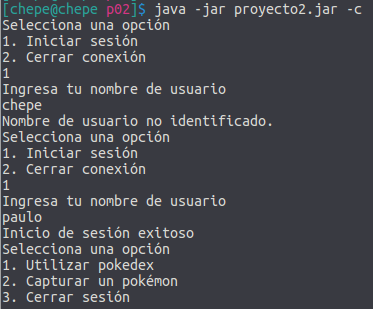
\includegraphics[width=0.5\textwidth]{01}
  \caption{Menú de inicio de sesión}
  \label{inicioSesion}
\end{figure}

En la interacción mostrada en la Figura \ref{inicioSesion}, se le pidió al usuario que escogiera entre iniciar sesión y cerrar la conexión. El cliente pidió iniciar sesión con el usuario \texttt{chepe} mandando el siguiente mensaje con código 10:
\begin{figure}[H]
  \centering
  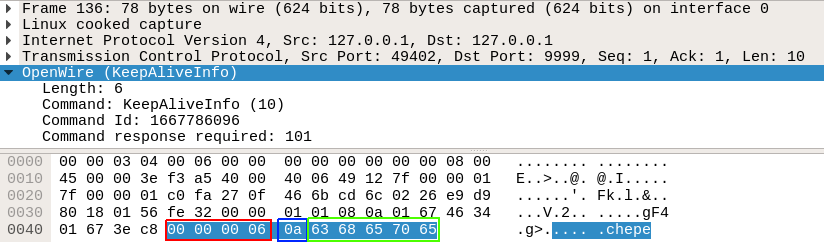
\includegraphics[width=\textwidth]{03}
  \caption{Mensaje con código 10}
\end{figure}

El servidor contestó con el mensaje de error con código 44, indicando que tal usuario no se encuentra registrado en la base de datos.
\begin{figure}[H]
  \centering
  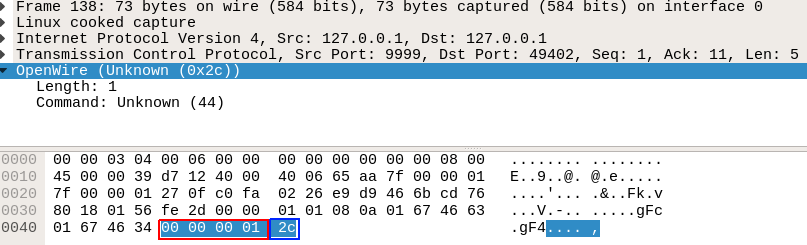
\includegraphics[width=\textwidth]{04}
  \caption{Mensaje de error con código 44}
\end{figure}

El cliente hace un segundo intento de inicio de sesión con un usuario distinto.

\begin{figure}[H]
  \centering
  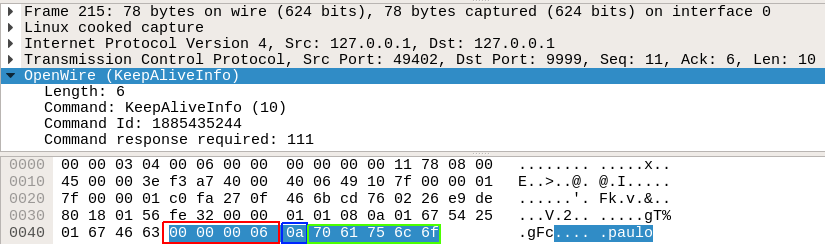
\includegraphics[width=\textwidth]{05}
  \caption{Mensaje con código 10}
\end{figure}

El servidor responde con el código 20, indicando que se inicio sesión exitosamente.

\begin{figure}[H]
  \centering
  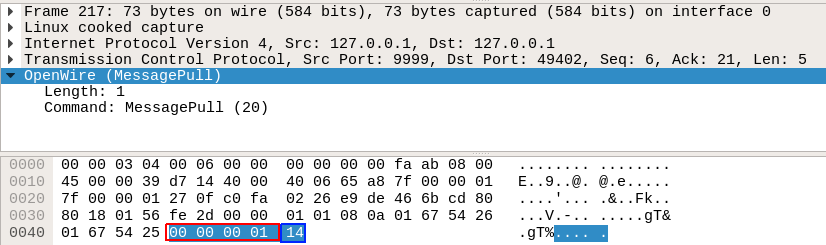
\includegraphics[width=\textwidth]{06}
  \caption{Mensaje con código 20}
\end{figure}

\subsubsection{Búsqueda de pokémon en Pokédex}

\begin{figure}[H]
  \centering
  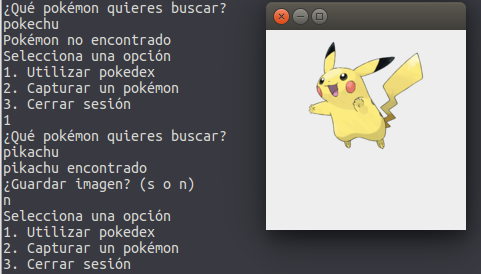
\includegraphics[width=0.5\textwidth]{07}
  \caption{Búsquedas en Pokédex}
\end{figure}

El cliente indica que quiere hacer una búsqueda del pokémon \texttt{pokechu} en su Pokédex.
\begin{figure}[H]
  \centering
  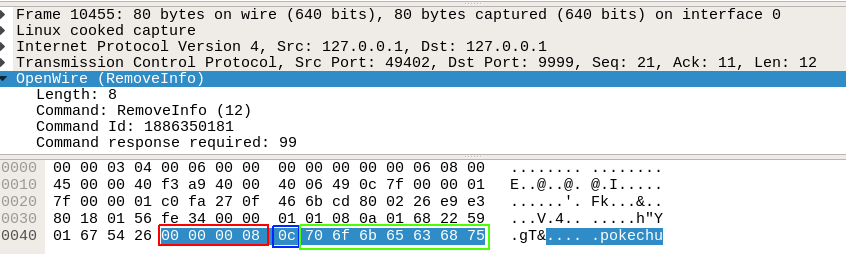
\includegraphics[width=\textwidth]{09}
  \caption{Mensaje con código 12}
\end{figure}

El servidor contesta con el código de error 44, indicando que no se encontró tal pokémon.
\begin{figure}[H]
  \centering
  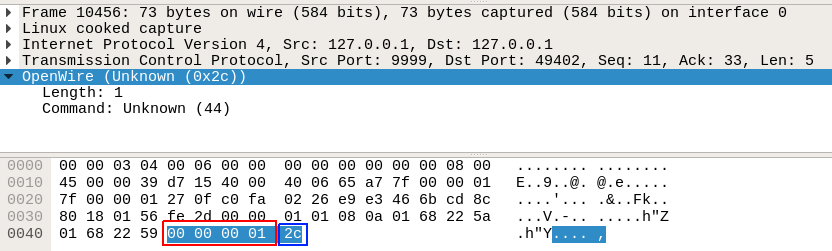
\includegraphics[width=\textwidth]{10}
  \caption{Mensaje con código de error 44}
\end{figure}

El cliente pide que se realice la búsqueda de otro pokémon, en este caso \texttt{pikachu}.

\begin{figure}[H]
  \centering
  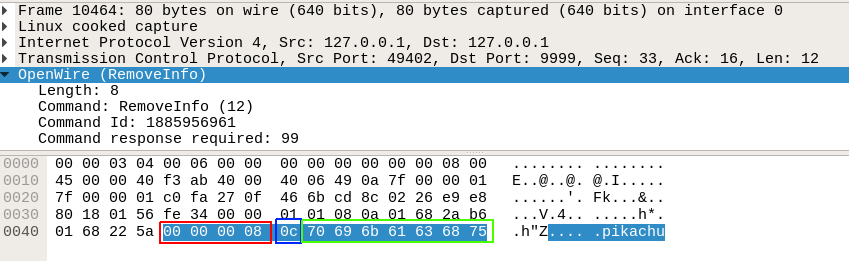
\includegraphics[width=\textwidth]{11}
  \caption{Mensaje con código 12}
\end{figure}

El servidor contesta con el código de éxito 21 junto con la imagen del pokémon, la cual se despliega en pantalla y se indica si se quiere guardar o no en el equipo del cliente.
\begin{figure}[H]
  \centering
  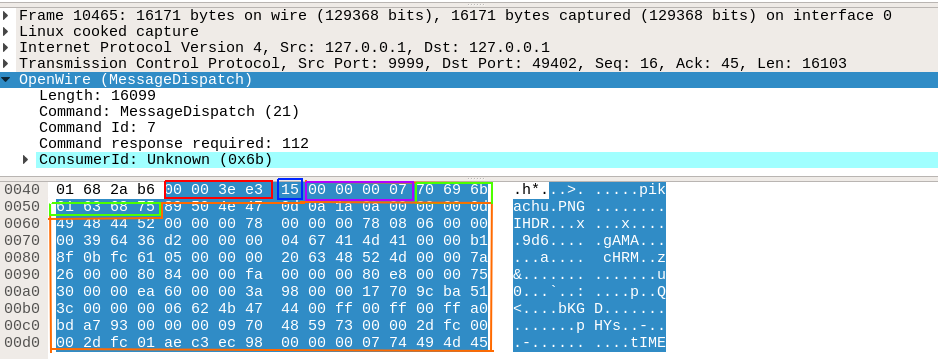
\includegraphics[width=\textwidth]{13}
  \caption{Mensaje con código 21}
\end{figure}

\subsubsection{Captura de un pokémon}

\begin{figure}[H]
  \centering
  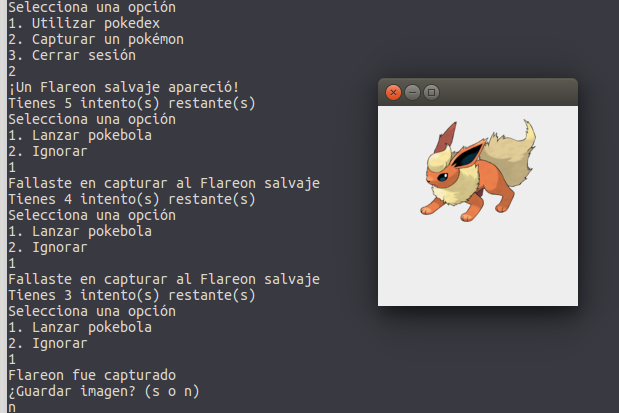
\includegraphics[width=0.5\textwidth]{14}
  \caption{Intentos de captura de un pokémon}
\end{figure}

El cliente pide capturar un pokémon.

\begin{figure}[H]
  \centering
  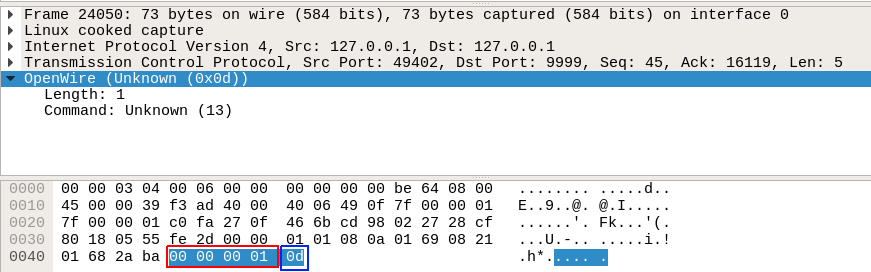
\includegraphics[width=\textwidth]{15}
  \caption{Mensaje con código 13}
\end{figure}

El servidor responde con un pokémon aleatorio, en este caso \texttt{Flareon}, y le da 5 intentos al cliente para capturar el pokémon.
\begin{figure}[H]
  \centering
  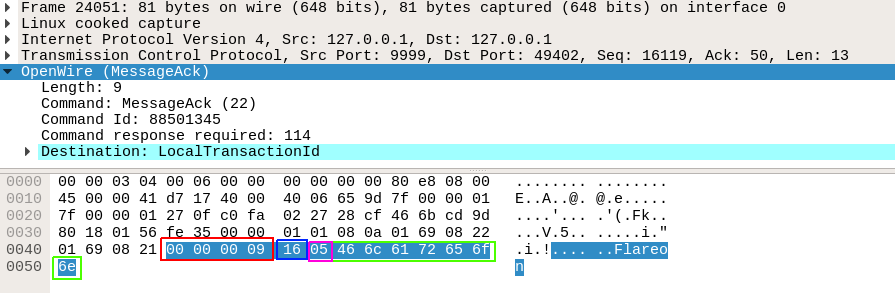
\includegraphics[width=\textwidth]{16}
  \caption{Mensaje con código 22}
\end{figure}

El cliente lanza su primer pokebola.
\begin{figure}[H]
  \centering
  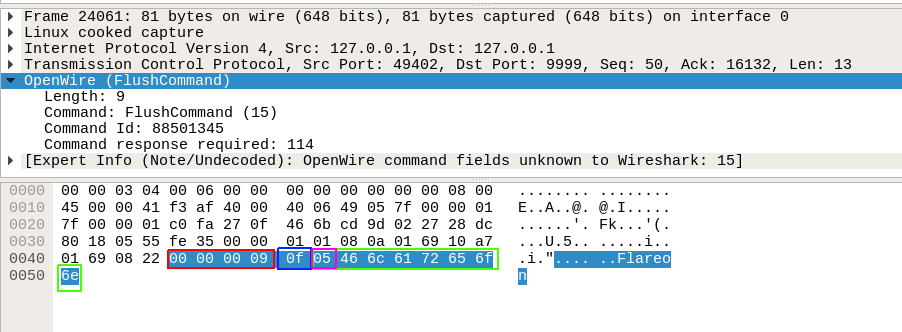
\includegraphics[width=\textwidth]{17}
  \caption{Mensaje con código 15; intento $\#$5}
\end{figure}

El servidor indica que falló el intento y decrementa el contador.
\begin{figure}[H]
  \centering
  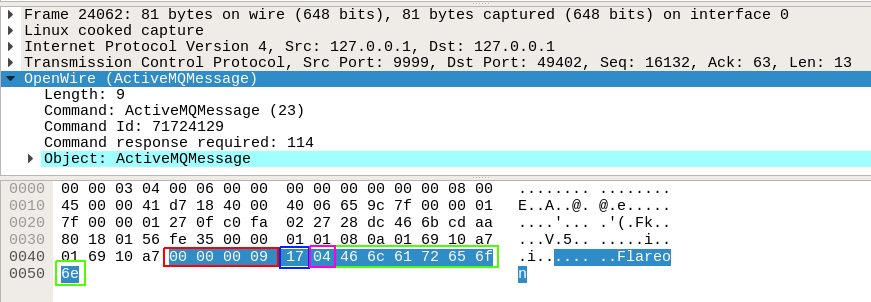
\includegraphics[width=\textwidth]{18}
  \caption{Mensaje con código 23; 4 intentos restantes}
\end{figure}

El cliente lanza otra pokebola.
\begin{figure}[H]
  \centering
  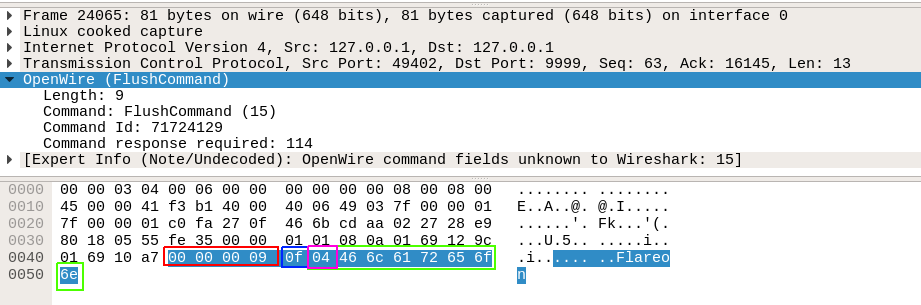
\includegraphics[width=\textwidth]{19}
  \caption{Mensaje con código 15; intento $\#$4}
\end{figure}

Se indica que de nuevo falló el lanzamiento, decrementa el contador.
\begin{figure}[H]
  \centering
  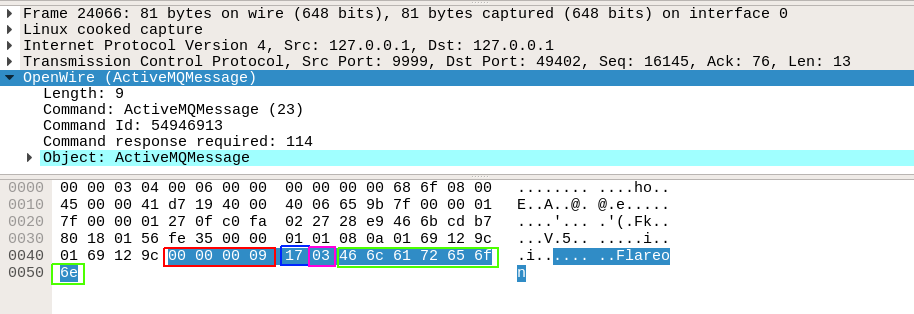
\includegraphics[width=\textwidth]{20}
  \caption{Mensaje con código 23; 3 intentos restantes}
\end{figure}

El cliente hace otro intento.
\begin{figure}[H]
  \centering
  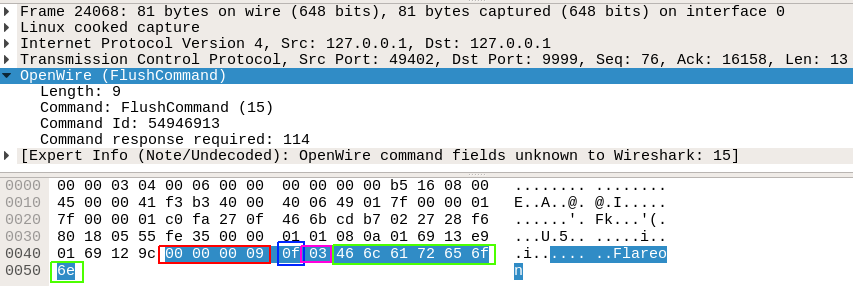
\includegraphics[width=\textwidth]{21}
  \caption{Mensaje con código 15; intento $\#$3}
\end{figure}

El servidor indica que esta vez sí se logró capturar el pokémon, y manda la imagen asociada a éste.
\begin{figure}[H]
  \centering
  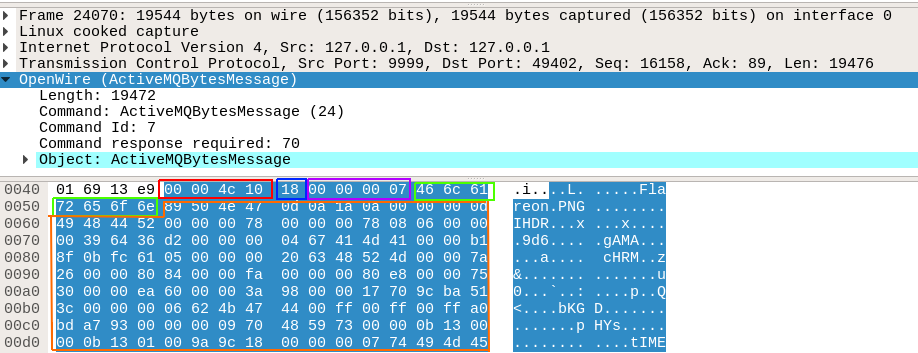
\includegraphics[width=\textwidth]{22}
  \caption{Mensaje con código 24}
\end{figure}

A continuación se muestra un caso en el que el cliente escoge ignorar al pokémon en vez de lanzar una pokebola.
\begin{figure}[H]
  \centering
  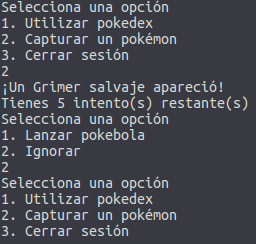
\includegraphics[width=0.3\textwidth]{23}
  \caption{Se ignora al pokémon Grimer}
\end{figure}

El cliente indica que quiere capturar un pokémon
\begin{figure}[H]
  \centering
  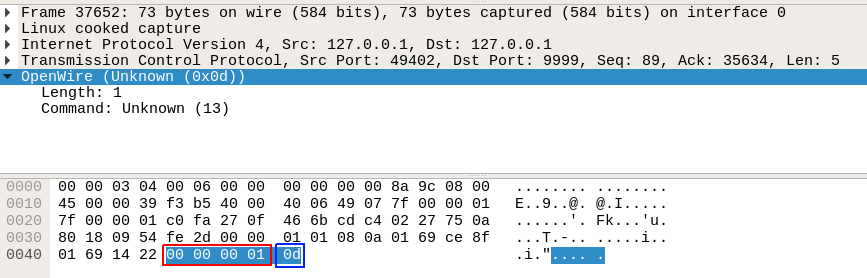
\includegraphics[width=\textwidth]{24}
  \caption{Mensaje con código 13}
\end{figure}

El servidor regresa al pokémon aleatorio \texttt{Grimer}.
\begin{figure}[H]
  \centering
  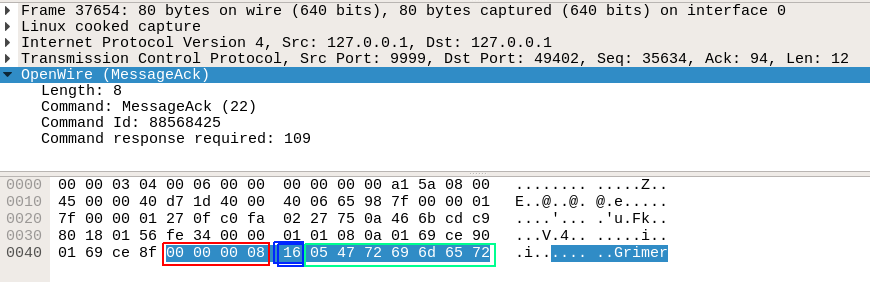
\includegraphics[width=\textwidth]{25}
  \caption{Mensaje con código 22}
\end{figure}

El cliente indica que no quiere capturar a tal pokémon.
\begin{figure}[H]
  \centering
  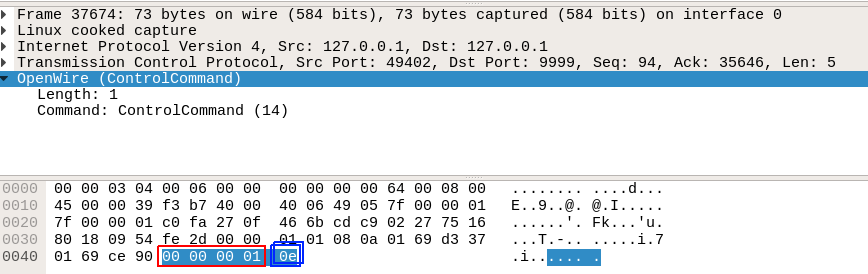
\includegraphics[width=\textwidth]{26}
  \caption{Mensaje con código 14}
\end{figure}

En el siguiente caso el cliente falla en el último intento de captura del pokémon \texttt{Magnemite}.
\begin{figure}[H]
  \centering
  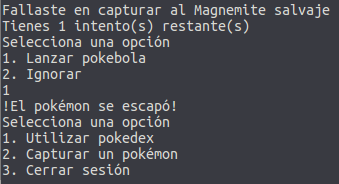
\includegraphics[width=0.5\textwidth]{27}
  \caption{}
\end{figure}

El cliente realiza el último intento para capturar a \texttt{Magnemite}.
\begin{figure}[H]
  \centering
  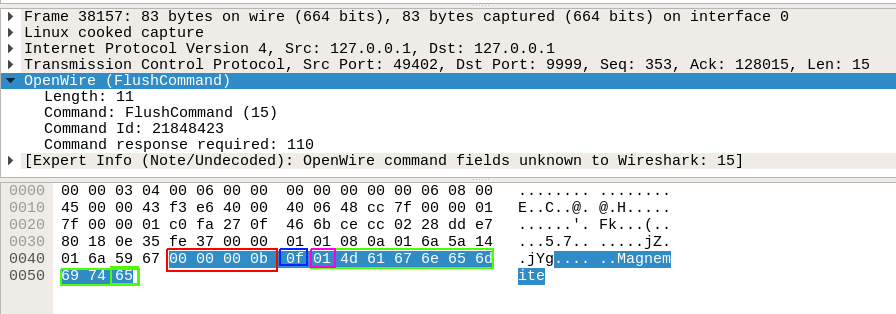
\includegraphics[width=\textwidth]{28}
  \caption{Mensaje con código 15; intento $\#$1}
\end{figure}

El servidor contesta con el código de error 41, indicando que el último intento de captura del cliente falló y ya no le quedan más intentos.
\begin{figure}[H]
  \centering
  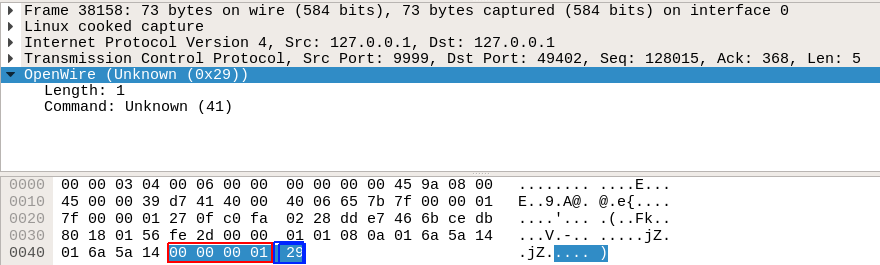
\includegraphics[width=\textwidth]{29}
  \caption{Mensaje con código de error 41}
\end{figure}

\subsubsection{Cierre de sesión y conexión}

\begin{figure}[H]
  \centering
  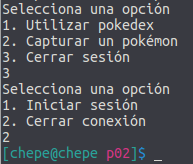
\includegraphics[width=0.3\textwidth]{30}
  \caption{El cliente cierra la sesión y se desconecta del servidor}
\end{figure}

El cliente manda un mensaje indicando que quiere cerrar sesión.
\begin{figure}[H]
  \centering
  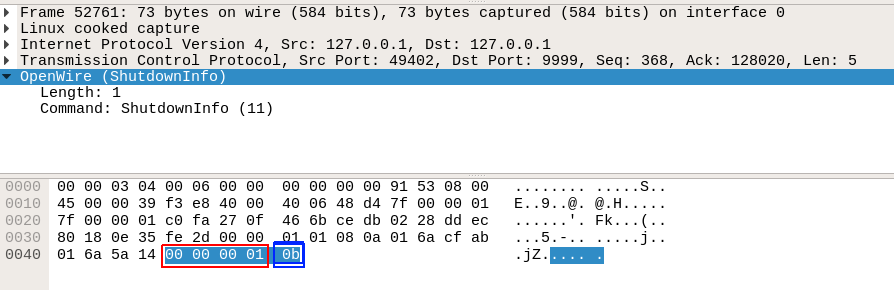
\includegraphics[width=\textwidth]{31}
  \caption{Mensaje con código 11}
\end{figure}

Posteriormente indica que también quiere cerrar la conexión con el servidor.
\begin{figure}[H]
  \centering
  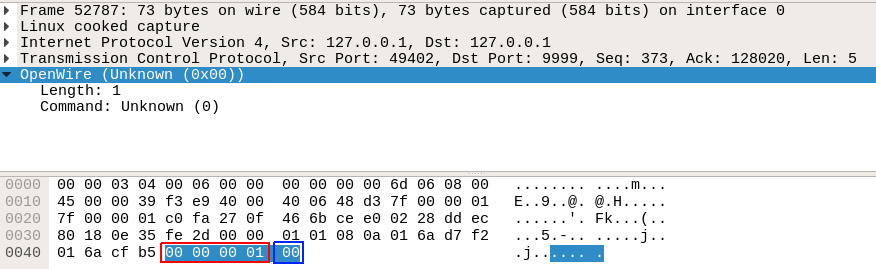
\includegraphics[width=\textwidth]{32}
  \caption{Mensaje con código 0}
\end{figure}


\end{document}
